\documentclass[12pt]{report}
\usepackage[utf8]{inputenc}
\usepackage[english]{babel}
\usepackage{graphicx}
\usepackage[autostyle]{csquotes}
\usepackage{amsmath}
\usepackage{subcaption}
\usepackage{array}
\newcolumntype{P}[1]{>{\centering\arraybackslash}p{#1}}
\usepackage[labelfont=bf]{caption}
\usepackage{indentfirst}
\graphicspath{{resources/}}
\usepackage[a4paper,width=150mm,top=25mm,bottom=25mm]{geometry}
\usepackage{fancyhdr}
\pagestyle{fancy}
\fancyhead{}
\lhead{Thesis Title}
\fancyfoot{}
\rfoot{\thepage}
\lfoot[LO,C]{Chapter \thechapter}
\renewcommand{\headrulewidth}{0.4pt}
\renewcommand{\footrulewidth}{0.4pt}

\newcommand{\quotes}[1]{\lq{#1}\rq}

% bibliography resources
\usepackage{biblatex}
\addbibresource{references.bib}

\title{Thesis Title}
\author{Austin Derrow-Pinion}
\date{October 2017}

\begin{document}

\begin{titlepage}
    \begin{center}
        \vspace*{0.4cm}

        \noindent\begin{minipage}{0.3\textwidth}
        
\includegraphics[width=\linewidth]{RoseSeal.png}
        \end{minipage}
        \hfill
        \begin{minipage}{0.6\textwidth}
        \raggedright\LARGE\bfseries
        Rose-Hulman Institute of Technology
        \end{minipage}

        \vspace*{1cm}

        \noindent\makebox[\linewidth]{\rule{\textwidth}{1pt}}\\
        \vspace{0.4cm}
        {\Huge \bfseries
        Thesis Title  % Thesis title
        \par}
        \vspace{0.4cm}
        \noindent\makebox[\linewidth]{\rule{\textwidth}{1pt}}

        \vspace{0.5cm}
        \LARGE
        Thesis Subtitle

        \vspace{1.5cm}

        \textbf{Austin Derrow-Pinion}

        \vfill

        \large
        \textit{
            In Partial Fulfillment of the\\
            Requirements for the Degree\\
            Bachelor of Science
        }

        \vspace{1cm}

        \Large
        Department of Computer Science \& Software Engineering\\
        Rose-Hulman Institute of Technology\\
        Terre Haute, Indiana\\
        October 2017\\
        Yosi Shibberu, Senior Thesis Advisor

    \end{center}
\end{titlepage}


\chapter*{Abstract}
Abstract content goes here...


\tableofcontents

\chapter{Introduction}
Memory augmented neural networks (MANN) have empowered neural networks with the
ability to solve problems that were previously unsolvable. The Neural Turing
Machine (NTM) \cite{DBLP:journals/corr/GravesWD14} is an early example of a
MANN. The NTM was greatly influenced by neuroscience research in working
memory. Later on, the Differentiable Neural Computer (DNC)
\cite{graves2016hybrid} was created as an enhancement of the architecture
in the NTM.


\chapter{Background}
Recurrent neural networks (RNNs) are Turing-Complete models that can perform
complex transformations on the data over an extended period of time
\cite{siegelmann1995computational}. Since RNNs are Turing-Complete, it is
evident that these models in theory can be used to solve any problems a
Turing machine can solve. However, a given problem may require a very specific
and complex setup of an RNN. Therefore we do not take the time to set up
RNNs manually in a way that it solves a specific problem. Rather, we design
rich architectures with the means of learning how to solve a problem in
an efficient manner. RNNs and models alike are trained using gradient descent
so that it solves a given problem with greater accuracy than before.

\section{Neural Turing Machines}
The Neural Turing Machine (NTM) is an RNN with a rich design that enables it to
learn how to solve problems better than basic RNNs. The NTM is an RNN with the
means of addressing a differentiable memory unit external to that of the model
itself \cite{DBLP:journals/corr/GravesWD14}.
Because of this differentiable memory unit, the model can learn what is most
important to store in memory. An efficient model would learn what information
is most useful and store that in memory to be read at a later timestep with the
assumption that the read results in a better solution to the task.
This creates a model that can more strongly refer to important imformation
that was present much earlier than a given timestep.

The NTM can be described as four main components: controller, read heads,
write heads, memory. The data flow of these four components is described
in Figure ~\ref{fig:NTMArchitecture}. Even though these components work in a
non-traditional manner, the model as a whole can be interacted with and
trained the same way you would any other RNN. The model simply receives
some external input at each timestep and will produce an external output
at each timestep. The components of the NTM are comparable to that of a
Turing machine, such that it contains read and write heads that interact
with a memory unit \cite{DBLP:journals/corr/GravesWD14}. Unlike a Turing
machine however, the NTM is end to end differentiable
\cite{DBLP:journals/corr/GravesWD14}. This feature gives the model a lot of
power in the field of Deep Learning research.

\begin{figure}[!htb]
    \centering
    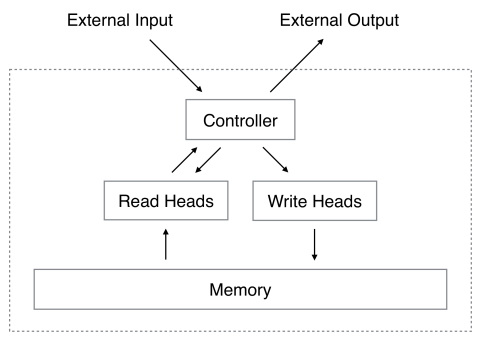
\includegraphics[width=0.9\linewidth]{resources/NTM.png}
    \caption{
        The components inside the dotted line represent everything the NTM
        is. The arrows represent the control flow of the data starting
        as \textit{External Input} fed into the \textit{Controller}. The
        \textit{Controller} can then activate either \textit{Read Heads} or
        \textit{Write Heads}. The \textit{Read Heads} do not receive any
        information about the \textit{External Input}, but is rather told what
        to read in \textit{Memory} by the \textit{Controller}. The
        \textit{Controller} can send information from the
        \textit{External Input} to the \textit{Write Heads} which then
        write that information into memory. The \textit{Controller} receives
        data back from the \textit{Read Heads} and then produces an
        \textit{External Output} \cite{DBLP:journals/corr/GravesWD14}.
    }
    \label{fig:NTMArchitecture}
\end{figure}

The memory unit is a matrix where the rows represent a memory location and the
number of columns correspond to how large each memory location is
\cite{DBLP:journals/corr/GravesWD14}. The read head emits a weighting vector
the length of the number of memory locations at each timestep
\cite{DBLP:journals/corr/GravesWD14}. A read operation on the memory matrix
is then a convex combination between this weighting and the contents of the
memory matrix \cite{DBLP:journals/corr/GravesWD14}. Using a weighting vector
here empowers the read head to narrowly focus on a single memory location's
information or to use a wider focus by using a little bit of information
from many different memory locations. The differentiability of the model allows
the read heads to learn the best weighting vectors to emit at a given state for
some timestep.

Writing to memory in the NTM is done with an erase operation followed by an
addition operation \cite{DBLP:journals/corr/GravesWD14}. The write head
emits three vectors at each timestep: \textit{weighting vector, erase vector,
add vector} \cite{DBLP:journals/corr/GravesWD14}. Assuming a weighting of $1$
for a memory location, a value of $1$ in the \textit{erase vector} at location
$j$ would mean to set the memory to $0$ in column $j$ within that memory
location \cite{DBLP:journals/corr/GravesWD14}. However, an
\textit{erase vector} with a value of $1$ can possibly not erase any
information in a memory location if the weighting for that memory location is
$0$ \cite{DBLP:journals/corr/GravesWD14}. So the \textit{erase vector}
represents the degree to which information in columns for weighted memory
locations shall be erased. As one would suspect, the \textit{add vector} works
quite oppositely from that of the \textit{erase vector}. Again assuming a
weighting of $1$ for a memory location, a value of $1$ in the
\textit{add vector} at location $j$ would mean to add $1$ to whatever value
is already stored in that memory location in column $j$
\cite{DBLP:journals/corr/GravesWD14}. Similarly to that of the
\textit{erase vector}, the weighting can overrule the \textit{add vector} by
having a value of $0$ for some location \cite{DBLP:journals/corr/GravesWD14}.
In other words, a value of $0$ in the \textit{weighting vector} means it does
not matter what the \textit{add vector} is because nothing will be added to
that memory location.

The weighting vectors emitted by both read and write heads are done so
through two different addressing mechanisms: \textit{content-based addressing},
\textit{location-based addressing} \cite{DBLP:journals/corr/GravesWD14}.
Content-based addressing compares a key vector with all of the memory locations
\cite{DBLP:journals/corr/GravesWD14}. This produces a weighting that has
greater values in locations that are most similar to that key vector and
lesser values in locations that are least similar to that key vector
\cite{DBLP:journals/corr/GravesWD14}. This addressing mechanism is useful for
easily identifying data in the memory matrix simply by producing an
approximation of that data. The location-based addressing mechanism is better
suited for iterating through sequence data or even jumping to a specific
memory location that may have a range of unknown data stored there. If the
previous weighting for a head was focused on location $j$, the location-based
addressing mechanism can easily produce a new weighting that focuses on
location $j-1$, $j$, or $j+1$. The choice between using these two addressing
mechanisms is controlled through a gating parameter emitted by the controller.
If this gating parameter is equal to $0$, then it will only use location-based
addressing. If the gating parameter is equal to $1$, then it will only use
content-based addressing. If the gating parameter is somewhere between
$0$ and $1$, it will use a mixture of both addressing mechanisms.

\section{Differentiable Neural Computers}
The Differentiable Neural Computer (DNC) is similar to that of the NTM, but
enhanced in it's ability to address the augmented external memory. These
enhancements make the DNC more capable than the NTM at solving complex,
structured tasks. Similarly to the NTM, the DNC is differentiable end-to-end
except one operation in which the researchers claim do not make a significant
impact on the model as a whole \cite{graves2016hybrid}.

A NTM is allowed any number of read and write heads, but the DNC limits
the number of write heads to be only one \cite{graves2016hybrid}. The NTM
was only able to iterate through consecutive written locations until a
content-based addressing write occured \cite{graves2016hybrid}. The DNC,
however, can continue iterating through consecutive written locations because
it has, what the researchers call, a temporal linkage matrix
\cite{graves2016hybrid}. The temporal linkage matrix, $L$, is $N \times N$ with
weighted values between zero and one \cite{graves2016hybrid}. A value closer
to one at position $(i, j)$ means memory location $i$ was written to directly
after memory location $j$ was written to \cite{graves2016hybrid}. Otherwise,
the value should be near zero \cite{graves2016hybrid}. So given a weighting
vector, $\bf{w}$, the vector produced by $L\bf{w}$ augments the weighting to
focus on memory locations written to directly \textit{after} those
locations focused on by weighting $\bf{w}$ \cite{graves2016hybrid}.
Conveniently, the vector produced by $L^\top \bf{w}$ augments the weighting to
focus on memory locations written to directly \textit{before} those
locations focused on by weighting $\bf{w}$ \cite{graves2016hybrid}. This
interaction between the temporal linkage matrix and the external memory is one
of the three differentiable attention mechanisms in the DNC
\cite{graves2016hybrid}. This attention mechanism replaces the location-based
addressing method from the NTM. The temporal linkage matrix allows the DNC to
better handle sequential data that is not necessarily written to in sequential
memory locations. This is a more powerful concept than that of the NTM's
location-based addressing mechanism which was limited to sequential
memory locations.

Like the NTM, the DNC uses a content-based addressing mechanism that produces
a weighting vector focusing on memory locations most similar to some
emitted key vector \cite{graves2016hybrid}. Similarity in both cases are
defined as cosine similarity
\cite{DBLP:journals/corr/GravesWD14,graves2016hybrid}. If the DNC controller
emits a key vector with only part of the information it needs, this
content-based addressing mechanism can be used to read the complete
information related to it. In theory this allows the DNC to iterate
through data structures in which memory locations reference other memory
locations through a key-value address mechanism.

Unlike the NTM, the DNC uses a \textit{usage vector} to find the best memory
locations to write to and to identify any important memory locations not to
write to \cite{graves2016hybrid}. The vector's values range between zero and
one, where values closer to one means the memory locations have greater usages
\cite{graves2016hybrid}. The weighting vector given to a write head focuses on
unused locations, where the usage vector has low values
\cite{graves2016hybrid}. When the write head writes to a memory location, the
usage vector is updated at that memory location by increasing the value
\cite{graves2016hybrid}. The usage vector is also capable of decreasing values
in a memory location after it is read \cite{graves2016hybrid}. For example,
consider a task which provides a sequence of numbers and then asks what that
sequence was. After asking for what a sequence was, it will provide a new
sequence of numbers and repeat itself. The DNC can learn to write that
sequence of numbers in the external memory using the write heads. At that
point, the usage vector will have greater values in those locations written
to and lower values in the locations not needed. When the task asks for the
sequence of numbers, the DNC would use the read heads to read those locations
written to. After the reads, the usage vector will update the memory locations
to have low usage. This effectively reallocates the memory locations for
later usage.

The DNC is very comparable to how a human interacts with what we think of as
a modern day computer. Much of the human interaction with computers are done
automatically with a trained DNC. For instance, a human controls more or less
exactly what to read and write in memory. The DNC however, learns what
information is most useful to read and write in memory without being controled
by an external force. When a human deletes data on a computer, they are
essentially reallocating space in their memory for future data to be stored.
In this same manner, the DNC automatically learns when to reallocate memory
based on the task given. So as the name suggests, the DNC can be thought of
as a differentiable computer. This does not mean that a DNC will ever take the
place of a modern day computer because the applications are different. When
we interact with a computer, we expect the memory to always be there regardless
of how often we may use it. Having the computer automatically erase data
because it thinks you do not need it would be very unfavorable for many users.
However, a DNC is a model that learns how to represent complex data
structures to solve difficult tasks that cannot otherwise be solved.

The DNC has been found to be useful in a variety of experimental applications.
The researchers show that the DNC outperforms the previous best models in
a synthetic question answering task using the bAbI dataset
\cite{graves2016hybrid}. The following example shows that the DNC is able to
combine supporting facts together to come up with a solution
\cite{graves2016hybrid}:
\begin{align*}
\textnormal{\bf{Input: }}  & \quad \textnormal{John is in the playground. John
                                               picked up the football.} \\
\textnormal{\bf{Input: }}  & \quad \textnormal{Where is the football?} \\
\textnormal{\bf{Output: }} & \quad \textnormal{playground.}
\end{align*}
An even more complex task is to still be able to combine supporting facts
but also have resilience to distractors in the input \cite{graves2016hybrid}:
\begin{align*}
\textnormal{\bf{Input: }}  & \quad \textnormal{Sheep are afraid of wolves.
                             Gertrude is a sheep.} \\
                           & \quad \textnormal{Mice are afraid of cats.} \\
\textnormal{\bf{Input: }}  & \quad \textnormal{What is Gertrude afraid of?} \\
\textnormal{\bf{Output: }} & \quad \textnormal{wolves.}
\end{align*}
This example requires the DNC to have textual reasoning and be able to ignore
the last sentence that is unecessary to answer the question. This shows that
the differentiable attention mechanisms in the DNC are working and capable
of handling complex tasks such as this.

To test how the DNC handles data structures, the researchers explored
performance on graph problems: \textit{traversal}, \textit{shortest path},
\textit{inference} \cite{graves2016hybrid}. Before the model was asked to solve
one of these problems, it would first receive a graph as input. The model would
learn how to represent this graph in external memory. When the model is asked
to complete a traversal task, it receives a starting node and a path in the
graph \cite{graves2016hybrid}. The model must then output the ending node of
the path, requiring a traversal through the graph \cite{graves2016hybrid}.
The shortest path problem was given by a start and end node
\cite{graves2016hybrid}. The model must output the in-order path from start to
end. The inference task is given by an incomplete triple
(\quotes{from node}, \quotes{to node}, \quotes{relation}), where one of the
three were missing \cite{graves2016hybrid}. For example, if \quotes{to node} is
missing from the input, the model must infer what node has the given
relationship with \quotes{from node}. In the example of a family tree, one
might ask (\quotes{Jen}, \quotes{\_}, \quotes{MaternalGreatUncle}). For which,
if Joe is Jen's Maternal-Great-Uncle, then the model is expected to output
the triple (\quotes{Jen}, \quotes{Joe}, \quotes{MaternalGreatUncle}). This task
requires the model to not only learn how to traverse the graphs, but to learn
the meaning of relationships.

When the three graph problems were tested on the DNC and a baseline LSTM, the
DNC produced much better results while the LSTM failed to even learn the
easiest task of traversal \cite{graves2016hybrid}. When tested on randomly
generated paths of length seven, the DNC performed with an accuracy of 98.8\%
and the LSTM performed with an accuracy of 37\% \cite{graves2016hybrid}. This
shows how the DNC can solve problems otherwise unsolvable because the DNC has
an external memory with read and write access. The DNC performed at an accuracy
of 55.3\% when tested on shortest paths of length four \cite{graves2016hybrid}.
On the last task, inference, the DNC performed with accuracy 81.8\% when tested
on relationships that connect nodes with distance four \cite{graves2016hybrid}.


\chapter{Procedures}
\section{Dynamic Memory Allocation}
Repeat-Copy is a task formulated in DeepMind's original DNC paper
\cite{graves2016hybrid} in order to test whether the architecture could
learn how to manage the external memory. The task itself isn't a difficult or
market demanding problem needing to be solved. The task simply has features in
which it can test the architecture of the DNC.

The Repeat-Copy task is described as follows. An agent receives as input
$n_{\textrm{min}}$ to $n_{\textrm{max}}$ sequences of $m$ many binary digits with
the task to repeat the sequences of binary digits a given $r_{\textrm{min}}$ to
$r_{\textrm{max}}$ many times. Consider an example when $n_{\textrm{min}} = 1$,
$n_{\textrm{max}} = 10$, $m = 4$, $r_{\textrm{min}} = 1$, and $r_{\textrm{max}} = 5$.
Then the agent would receive between 1 to 10 sequences of 4 binary digits with
the task of repeatedly outputing those sequences of 4 binary digits between 1
to 5 times. An equivalent task to this example would be to ask the agent to
output the following matrix 5 times:
$$
\begin{bmatrix}
    0 & 1 & 0 \\
    1 & 1 & 1 \\
    0 & 0 & 1 \\
    0 & 1 & 1
\end{bmatrix}
$$
where each of the $n$ many columns represent a sequence of $m$ binary digits.
The results reported by DeepMind's DNC \cite{graves2016hybrid} are on this
problem where $n_{\textrm{min}} = n_{\textrm{max}} = 5$, $m = 6$, and
$r_{\textrm{min}} = r_{\textrm{max}} = 1$.

The free gate in the DNC is active when the most recently read locations in
external memory can be freed. The allocation gate governs the strength to which
locations in external memory can be reused for new data. Training the DNC on
the Repeat-Copy task is forcing the model to learn when to free limited
external memory and reuse that freed memory to best take advantage of it.
Consider a task where the DNC receives a sequence of 10 random binary digits as
input and must repeat those 10 random binary digits as output. If the DNC uses
a feed-forward network with only an external memory of 10 locations, it must
learn to use the memory to only store data for each sequence at a time. The
DNC in this case doesn't have enough memory space to store all input it
receives to repeat. The results reported by DeepMind's DNC paper
\cite{graves2016hybrid} are such that the DNC learned how to manage external
memory as we would expect it must in order to succeed at the task. The free
gate became active while reading from external memory to immediately make that
space available for writing later. The allocation gate became active while
receiving input to write the input into the freed locations.

The purpose of repeating DeepMind's Repeat-Copy results \cite{graves2016hybrid}
in my implementation has two primary reasons. Firstly, to reconfirm the ability of
the DNC to learn how to manage memory efficiently. Secondly, to ensure my
implementation of the DNC behaves similar to that of DeepMind's before
attempting further tasks. My results are shown in Figure ~\ref{fig:repeatCopyResults}
and successfully repeat the same results reported by DeepMind's implementation
\cite{graves2016hybrid}.

\begin{figure}[h]

\includegraphics[width=0.4\textwidth]{../resources/RoseSeal.png}
\caption{My results on the Repeat-Copy task (image is a placeholder).}
\label{fig:repeatCopyResults}
\end{figure}


\section{DNA Sequencing for Pre-Segmented MinION Nanopore Reads}
DNA sequencing methods first starting publishing in 1975 \cite{SANGER1975441}.
In 1977, the Sanger method was shown to be the fastest and most accurate
way to sequence DNA at the time \cite{sanger1977dna}. Since then, the
Human Genome Project (HGP) has started with the goal of sequencing and mapping
the entire human genome \cite{international2001initial}. The HGP helps
accelerate biomedical research by providing a mass amount of data
that can be used to locate disease genes, identify drug targets, or even
research other physiology and cell biology applications
\cite{international2001initial}. In summary, DNA sequencing is not only
beneficial for research purposes, but also beneficial for clinical purposes.

MinION is a USB memory stick sized device from Oxford Nanopore Technologies
costing approximately \$1000 and produces DNA sequence data using nanopores.
The nanopores produce signals which we can segment into groups. Base-calling
algorithms classify these groups into nucleotides (\textit{A}, \textit{G},
\textit{C}, or \textit{T}). As DNA fragments are fed through the device,
a drop in electrical current occurs depending on the nucleotide in the
nanopore. These drops in electrical current are recorded in a series of
signals. A base-caller algorithm then must read these recorded signals and
produce the corresponding DNA sequence.

The base-caller, DeepNano, is built using a recurrent neural network and has
been found to perform more accurately than the default base caller supplied
by the manufacturer \cite{bovza2017deepnano}. DeepNano achieved 77.9\% accuracy
on an \textit{E. coli} dataset and 76.3\% accuracy on a \textit{K. pneumoniae}
dataset \cite{bovza2017deepnano}. The default base caller, Metrichor, only
achieved 71.3\% accuracy on the \textit{E. coli} dataset and 68.1\% accuracy on
the \textit{K. pneumoniae} dataset \cite{bovza2017deepnano}.

We test the performance of the DNC as a base caller on a MinION dataset
provided by Ryan Poplin on the Google Brain team. The dataset consists of a
\texttt{train.hdf5} file with size 2.9 GB and a \texttt{val.hdf5} file with
size 1.16 GB. Each file has multiple hdf5 groups representing a run of the
MinION device. A group in one of the hdf5 files has both a \quotes{label} and a
\quotes{signal} dataset. The \quotes{signal} dataset contains the signals
generated by the MinION device. The \quotes{label} dataset is a collection
of triples \mbox{(\quotes{start index}, \quotes{end index}, \quotes{base})}.
The signals at indices \mbox{[\quotes{start index}, \quotes{end index}]} are
labelled as the nucleotide \quotes{base}.

We used an LSTM as a baseline model to compare performance on the dataset with
the DNC. We tested four different LSTM models differing on the number of units
used. Table \ref{tab:table3_1} shows the results of the LSTM baseline models.
The best LSTM performance on the validation dataset was with X many units.
The testing accuracy for the model with X many units is reported on a dataset
of size X from the \texttt{val.hdf5} file (0.00\%).

\begin{table}[h!]
\begin{center}
\begin{tabular}{ | c || c | c | }
 \hline
 \multicolumn{3}{|c|}{\bf{LSTM Baseline Model Performances}} \\
 \hline
 Number of Units & Training Accuracy & Validation Accuracy \\
 \hline
 128  & 0.00\% & 0.00\% \\
 512  & 0.00\% & 0.00\% \\
 1024 & 0.00\% & 0.00\% \\
 2048 & 0.00\% & 0.00\% \\
 \hline
\end{tabular}
\caption{
    All LSTM models were trained on a dataset with size X from
    the \texttt{train.hdf5} file. Each model trained for X many training
    iterations. Accuracy is defined as the number of correctly labeled
    nucleotides divided by the number of total nucleotides labelled. Validation
    accuracy is reported on a validation set of size X from the
    \texttt{train.hdf5} file.
}
\label{tab:table3_1}
\end{center}
\end{table}

The DNC was trained on the same datasets as the LSTM baseline models. A subset
of the total grid search method was used for hyperparameter optimization.
Results for the five best trained models are shown in Table \ref{tab:table3_2}.
Training the best performing DNC model for an additional 50,000 steps resulted
in a training accuracy of 85\% and a validation accuracy of 37\%. This is
almost the same as when the model was only trained with 100,000 iterations and
thus we can conclude training longer will not result in any improvements.

\begin{table}[h!]
\begin{center}
\begin{tabular}{ | c | c | c || P{2cm} | P{2cm} | }
 \hline
 \multicolumn{5}{|c|}{\bf{DNC Performance on DNA Sequencing}} \\
 \hline
 Read Heads & Memory Size & Word Size & Training Accuracy & Validation Accuracy \\
 \hline
 4  & 16 & 4  & \bf{90\%} & \bf{38\%} \\
 16 & 128& 64 & 35\% & 37\% \\
 1  & 8  & 1  & 46\% & 32\% \\
 1  & 32 & 16 & 33\% & 27\% \\
 8  & 32 & 16 & 27\% & 26\% \\
 \hline
\end{tabular}
\caption{
    \textbf{Table 3.2:} All DNC models were trained on a dataset with size 100
    from the \texttt{train.hdf5} file. Each model trained for 100000 many
    training iterations. Accuracy is defined as the number of correctly labeled
    nucleotides divided by the number of total nucleotides labelled. Validation
    accuracy is reported on a validation set of size 10000 from the
    \texttt{train.hdf5} file.
}
\label{tab:table3_2}
\end{center}
\end{table}

Using a training dataset size of 10000, we trained a DNC model with the same
hyperparameters as the best performing model in Table \ref{tab:table3_2}:
four read heads, memory size of sixteen, word size of four. After 100000
training iterations, the model was performing with a training accuracy of
53\% and a validation accuracy of 29\%. After training an additional 50000
iterations, the training accuracy went down to 51\% and the validation
accuracy went to 30\%. Due to the difference in validation accuracy being only
1\% and the training accuracy decreasing, we conclude further training the
model would result in no further significant improvements. The DNC model
performed with greater accuracy when trained with only 100 examples.

We have found that the DNC model is unable to perform DNA sequencing on
nanopore reads at the accuracy of other available software as described
previously. Future research may reveal that a different subset of training data
and a different configuration of hyperparameters yields a better performing
DNC on the task.


% \chapter{Extraction-Based Summarization Task}
% Automatic summarization is a term used to describe the action of processing
some text to output some form of a meaningful summary in a representative
manner. Extraction-based summarization is a type of automatic summarization in
which the goal is to extract key-terms as the summary of some text.

As a novel application for the DNC, I applied it to the extraction-based
summarization task of generating tags from Stack Exchange questions. I obtained
a dataset from the Facebook Recruiting III - Keyword Extraction\footnote{can be
found at https://www.kaggle.com/c/facebook-recruiting-iii-keyword-extraction/}
competition on Kaggle. The training dataset contains 6,034,195 questions and
the testing dataset contains 2,013,337 questions. The correct answers for the
testing dataset are not publicly available, but submissions can still be scored
on the Kaggle competition. Scores reported for this task are mean F-scores as
determined by the Kaggle submission report. For example, $1.0$ means a perfect
score and $0.0$ means nothing correct at all. When the competition was live
four years ago (August 30, 2013), the winner received a score of $0.81350$.

Each question contains three main features: title, question, tags. The training
dataset includes all three features while the testing dataset only contains the
title and question features. Below is an example from the training dataset:
\blockquote{
\textbf{Title:} How to check if an uploaded file is an image without mime type?
\\ \\
\textbf{Question:} {\textless}p{\textgreater}I'd like to check if an uploaded
file is an image file (e.g png, jpg, jpeg, gif, bmp) or another file. The
problem is that I'm using Uploadify to upload the files, which changes the mime
type and gives a 'text/octal' or something as the mime type, no matter which
file type you upload.%
{\textless}/p{\textgreater}{\textbackslash}n{\textbackslash}n%
{\textless}p{\textgreater}Is there a way to check if the uploaded file is an
image apart from checking the file extension using PHP?%
{\textless}/p{\textgreater}{\textbackslash}n
\\ \\
\textbf{Tags:} php image-processing file-upload upload mime-types}
The data comes directly from user-posted questions with only anonymization
changes. The length of the features can all be different for each question. The
goal for the testing dataset is to receive the title and question features as
input and output the tags feature.


\chapter{Conclusion}
Conclusion content goes here...


% \appendix
% \chapter{Appendix Title}
% Appendix content goes here...


\printbibliography

\end{document}
